\chapter{Sequences}


\section{What is a Sequence}
\subsection{Definition}
A sequence is a list of numbers in a specified order. The different numbers occurring in a sequence are called the terms of the sequence.\\
\[
    a_1,a_2,a_3,a_4\ldots,a_n
\]
Where the first term of the sequence is $a_1$, second term is $a_2$, n'th term is $a_n$.
We write a sequence using these notations:\\
\[
    a_n , \; (a_n), \; \{a_n\}, \; \{a_n\}_{n=1}^\infty
\]
Examples:\\
\begin{enumerate}
    \item $a_n = n = 1,2,3,4,\ldots$
    \item $a_n = n^2 = 1,4,9,16,\ldots$
    \item $a_n = (-1)^{n+1} = 1,-1,1,-1,\ldots$
    \item $a_n = \frac{1}{n} = 1,\frac{1}{2},\frac{1}{3},\frac{1}{4},\ldots$
    \item $a_n = \frac{(-1)^{n+1}}{n} = 1,-\frac{1}{2},\frac{1}{3},-\frac{1}{4},\ldots$
    \item $a_n = 1$ if $n$ is even, $n$ if $n$ is odd $= 1,1,3,1,5,1,7.\ldots$
    \item $a_n = 2,3,5,7,11,13,\ldots\;$ this is the sequence for prime numbers, it does not have a formula!
\end{enumerate}



\section{Limit Of A Sequence}
\subsection{Definition}
$L$ is the limit of a sequence $a_n$, or $a_n$ approaches $L\;$,$\lim_{n\to \infty} a_n = L,\: a_n\rightarrow L \iff$\\
$\forall\: \varepsilon>0 \:, \exists \: N\in \R,$ such that $\forall \: n>N \Longrightarrow |a_n - L|<\varepsilon$\\
Some people might be reading this and thinking what is all of this, so i'm gonna translate it for you.
For any positive number let's call it $\varepsilon$, there exists a number let's call it $N$ such that for any index that is bigger than that number $(N)$ the following happens $\Longrightarrow |a_n-L|<\varepsilon$, this is a literal translation from maths to english.\\\\


\subsection{Understanding The Limit}
Given any positive number $\varepsilon$, there exists a number $N$ such that for all indexes bigger than $N$ all the terms of the sequence apply this:\\
\[
    |a_n-L|<\varepsilon
\]
Which also means:
\[
    -\varepsilon<a_n-L<\varepsilon \quad \textbf{Feature 8}
\]
\[
    \iff
\]
\[
    L-\varepsilon<a_n<L+\varepsilon
\]
which means after a certain number $N$ all the terms of the sequence are going to be located between $L-\varepsilon$ and $L+\varepsilon$ or, $\forall \; \varepsilon>0 \; \exists \; N,$ such that $\forall\; n>N \Longrightarrow a_n\in (L-\varepsilon,L+\varepsilon)$



\subsection{Visually Seeing The Limit}
\noindent Examples:\\
If we look at the sequence $a_n = \frac{1}{n} = 1,\frac{1}{2},\frac{1}{3},\ldots$ we can tell that it approaches $0$, because the fractions are getting smaller and smaller each term.\\
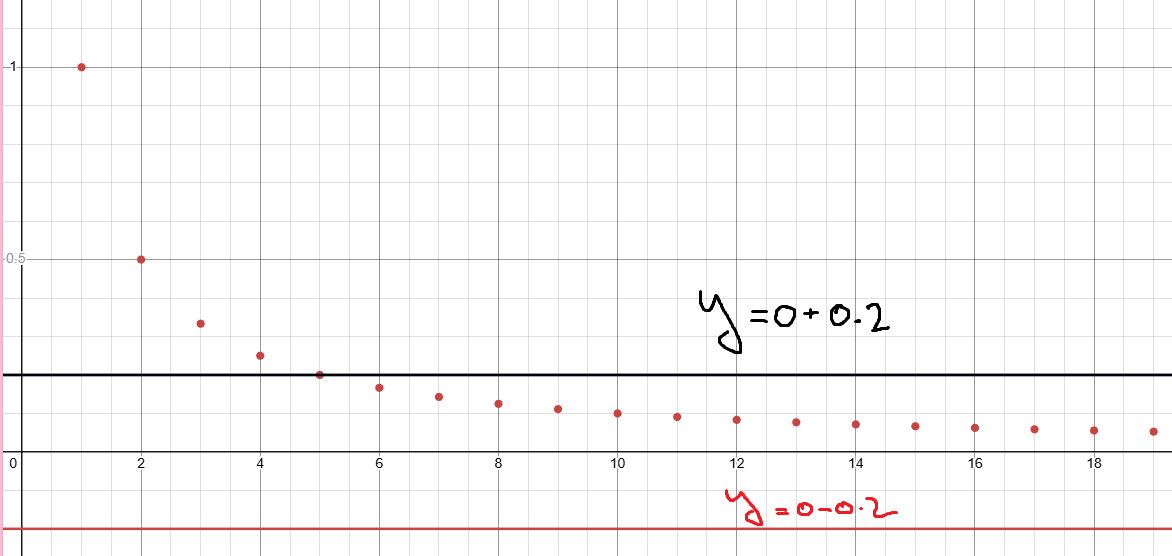
\includegraphics[scale = 0.7]{pictures/Graph1.png}
Given an $\varepsilon = 0.2$ $\exists\; N = 5,$ such that for all indexes bigger than $5\\ \Longrightarrow$ $0-0.2<a_n<0+0.2$\\
The definition of a limit states, that given any positive number $\varepsilon$, therefor we can pick any positive number $\varepsilon$ no matter how big and small it is, and there is always going to be a number $N$ such that for all the indexes bigger than $N$ such that $a_n\in(0-\varepsilon,0+\varepsilon)$\\\\
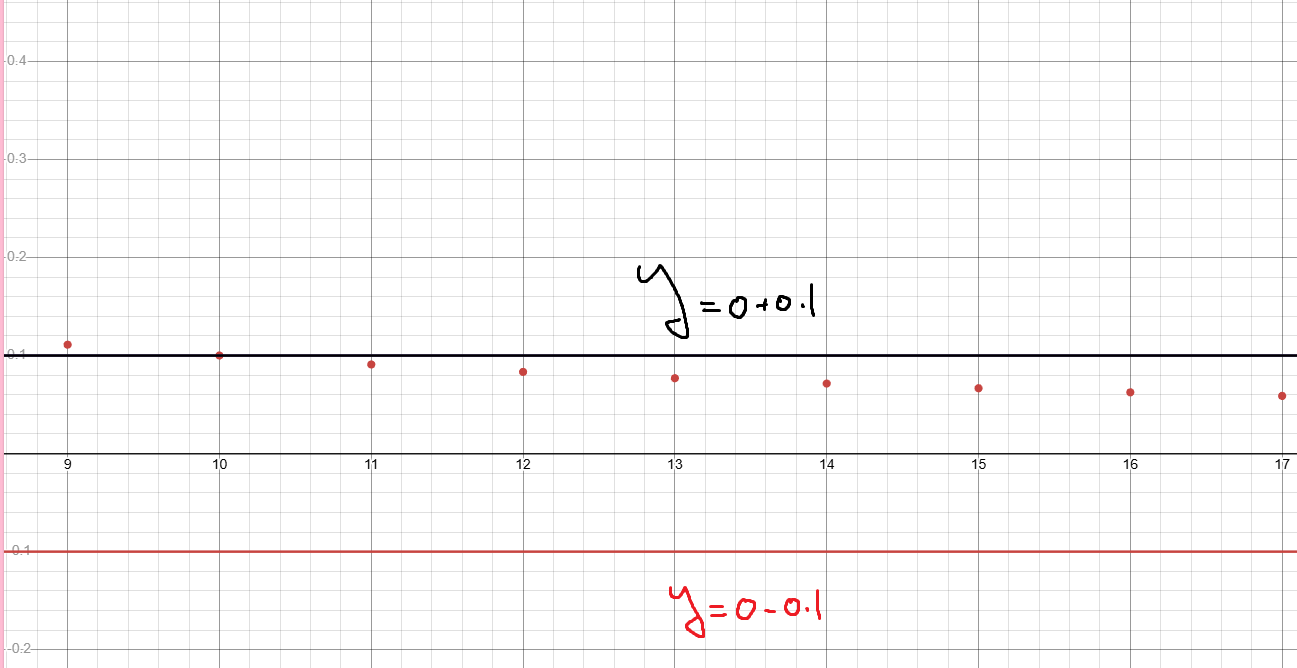
\includegraphics[scale=0.7]{pictures/Graph2.png}
Given an $\varepsilon = 0.1$ $\exists\; N = 10,$ such that for all indexes bigger than $10\\ \Longrightarrow$ $0-0.1<a_n<0+0.1$

\subsection{How To Prove The Limit Of A Sequence Is L}
In order to prove $\lim_{n\to \infty} a_n = L$, a sequence $a_n$ approaches $L$, we first have to understand how the definition of a limit works.\\
In basic terms:\\
For any positive number let's name it $\varepsilon$, exists a number let's name it $N\ldots$\\
Meaning we have to prove exists a number $N$ such that for all the indexes(n) bigger than $N\Longrightarrow$\\
\[
    |a_n-L|<\varepsilon
\]
We prove something exists finding out it's value, meaning we have to find the value of $N$.\\
Here is how i like to prove these type of questions, which are to prove that a sequence $a_n$ approaches $L$, or for short $\lim_{n\to\infty}a_n=L,\;a_n\rightarrow L$\\



\subsubsection{Question 1: Proving \(\lim_{n \to \infty} \frac{1}{n} = 0\)}
At first i like to write down the definition of an approaching sequence (Almost)\\
$\forall \; \varepsilon>0,\; \exists \; N = \square ,$ such that $\forall \; n>N \Longrightarrow$\\
as you can see so far all good, but i did not write what $N$ is equal to, i leave it blank, because i do not know it's value yet.\\
just so you remember, we want to  because prove:\\
$\forall \; \varepsilon>0, \; \exists\; N,$ such that $\forall \; n>N \Longrightarrow$
\[
    |a_n-L| = |\frac{1}{n}-0|<\varepsilon
\]
In the definition we say that $N$ exists, but we don't know what it is in this scenario, that's what we're going to find.\\
$\forall \; \varepsilon>0,\; \exists \; N = \square ,$ such that $\forall \; n>N \Longrightarrow$
\[
    |\frac{1}{n} - 0| = \frac{1}{n}<\frac{1}{N}
\]
Because we're looking for all $n>N$, meaning we're looking at terms that are bigger than $N$, if $n>N$, then $\frac{1}{n}<\frac{1}{N}$\\
now if $\frac{1}{N} = \varepsilon$ then $\frac{1}{n}<\varepsilon$ and $|\frac{1}{n}-0| <\varepsilon$.\\
$\frac{1}{N} = \varepsilon \iff N=\frac{1}{\varepsilon}$, now sub in $N = \frac{1}{\varepsilon}\:$, here's what the reader is gonna see.\\

\noindent$\forall \; \varepsilon>0,\; \exists \; N = \frac{1}{\varepsilon} ,$ such that $\forall \; n>N \Longrightarrow$\\
\[
    |\frac{1}{n}-0|=\frac{1}{n}<\frac{1}{N} = \varepsilon
\]



\subsubsection{Question 2: Proving \(\lim_{n \to \infty} c = c\)}
Given a sequence $a_n = c ,\; c\in \R\;$ a constant sequence, we need to prove that $\lim_{n\to\infty}a_n = c$.\\
as we said we first write the definition while leaving $N$ blank to fill it in when we find it.\\
$\forall \; \varepsilon>0,\; \exists \; N = \square ,$ such that $\forall \; n>N \Longrightarrow$\\
\[
    |c-c| = 0 <\varepsilon
\]
for any input$(n)$, therefor $N$ can be any number, let's pick $1$
here's what the reader is gonna see after you fill in for $N=1$\\
$\forall \; \varepsilon>0,\; \exists \; N = 1 ,$ such that $\forall \; n>N \Longrightarrow$\\
\[
    |c-c|=0<\varepsilon
\]



\subsubsection{Question 3: Proving \(\lim_{n \to \infty} \frac{3n^2-5n+4}{n^2+4n-5} = 3\)}
Given the sequence $a_n = \frac{3n^2-5n+4}{n^2+4n-5},\;$ we need to prove that $\lim_{n\to\infty}a_n = 3$\\
Again, we start by writing the definition of a limit while leaving $N$ blank to fill it in when we find it.\\
$\forall\; \varepsilon>0\; \exists\;N = \square ,$ such that $\forall\; n>N\Longrightarrow$\\
\textbf{1st Step: Simplify The Expression}
\[
    |\frac{3n^2-5n+4}{n^2+4n-5}-3| = |\frac{3n^2-5n+4}{n^2+4n-5} -3\cdot\frac{n^2+4n-5}{n^2+4n-5}|=|\frac{3n^2-5n+4-3n^2-12n+15}{n^2+4n-5}|
\]
\[
    |\frac{-17n+19}{n^2+4n-5}| =|\frac{-1\cdot(17n-19)}{n^2+4n-5}| = |-1|\cdot|\frac{17n-19}{n^2+4n-5}| = |\frac{17n-19}{n^2+4n-5}| \quad \textbf{(Feature 5)}
\]
\textbf{2nd Step: Get Rid Of The Absolute Value}\\
We get rid of the Absolute Value by making whatever is inside the Absolute Value positive, \textbf{Reminder}: $|a| = a \iff a \geq 0$\\
If we look at a fraction $\frac{a}{b},\; b\neq 0$, if $a$ gets bigger, then the fractions it self gets bigger.\\
For all $n>2\Longrightarrow 17n-19>0 \Longrightarrow |17n-19|=17n-19<17n$
\[
    \Longrightarrow |\frac{17n-19}{n^2+4n-5}|=\frac{17n-19}{|n^2+4n-5|}<\frac{17n}{|n^2+4n-5|}
\]
For all $n>2$ the denominator $n^2+4n-5>0\Longrightarrow |n^2+4n-5| = n^2+4n-5$\\
$\forall\; n>2\Longrightarrow 4n-5>0 \iff n^2+4n-5>n^2\iff \frac{1}{n^2+4n-5}<\frac{1}{n^2}$ 
\[
    \frac{17n}{|n^2+4n-5|}<\frac{17n}{n^2}=\frac{17}{n}
\]
Where are looking for all the indexes $(n)>N \iff \frac{1}{n}<\frac{1}{N}$
\[
    \frac{17}{n}<\frac{17}{N}
\]
If $\frac{17}{N} = \varepsilon$ then the inital term $|\frac{3n^2-5n+4}{n^2+4n-5}-3|<\varepsilon \Longrightarrow \frac{17}{N}=\varepsilon \iff N=\frac{17}{\varepsilon}$
\[
    \frac{17}{n}<\frac{17}{N}<\varepsilon
\]
\textbf{3rd Step: Picking N}\\
All of this works if all the indexes are bigger than $2$, so we can't say that $N=\frac{17}{\varepsilon}$ is a valid answer, because we're saying that this statment works for every positive number $\varepsilon$, some values for $\frac{17}{\varepsilon}$ are less than $1$.\\
There is a solution for this.\\
$\forall\; \varepsilon>0 ,\; \exists\; N=max\{\frac{17}{\varepsilon},2\},$ such that $\forall\; n>N\Longrightarrow$
\[
    |\frac{3n^2-5n+4}{n^2+4n-5}-3|<\ldots<\frac{17}{N}=\varepsilon
\]
If $\frac{17}{\varepsilon}>2$ then if $N = \frac{17}{\varepsilon}\Longrightarrow |\frac{3n^2-5n+4}{n^2+4n-5}-3|<\varepsilon$\\
Otherwise, meaning if $\frac{17}{\varepsilon}\leq 2 \iff \frac{17}{2}\leq \varepsilon$ and for $N=2\Longrightarrow \frac{17}{N}=\frac{17}{2}\leq \varepsilon$\\



\section{The Limit Of A Sequence Is Unique}
\subsection{Proof In Plain English}
If a sequence has a limit, then it is \textbf{Unique}. Before we got to the mathematical proof, i'm gonna explain in plain english using the knowledge we know so far to prove how the limit of a sequence is unique.\\
Given a sequence $a_n\rightarrow L,$ Using the definition of a limit: $\forall\; \varepsilon>0,\; \exists\; \N>0,$ such that for all indexes$(n)$ bigger than $N\Longrightarrow$
\[
    |a_n-L|<\varepsilon \iff a_n\in (L-\varepsilon,L+\varepsilon) \equiv L-\varepsilon<a_n<L+\varepsilon
\]
Meaning after a certain point $N$ every term of the sequence $a_n$ is in 
\[
    |a_n-L|<\varepsilon\; \equiv\; L-\varepsilon<a_n<L+\varepsilon\\
\]
If there are two limits $(L,K), L<K$, then the sequence is gonna be approaching two limits $L$ and $K$.\\
\textbf{First Limit}\\
$a_n\rightarrow K \Longrightarrow \forall \; \varepsilon>0, \exists\; N_1,$ such that $\forall n>N_1 \Longrightarrow$
\[
    |a_n-K|<\varepsilon \iff K-\varepsilon<a_n<K+\varepsilon
\]
\textbf{Second Limit}\\
$a_n\rightarrow L \Longrightarrow \forall \; \varepsilon>0, \exists\; N_2,$ such that $\forall n>N_2 \Longrightarrow$
\[
    |a_n-L|<\varepsilon \iff L-\varepsilon<a_n<L+\varepsilon
\]
\textbf{The Definition Of A Limit} states that $\forall\; \varepsilon>0\; \exists\; N,$ such that $\forall\; n>N\Longrightarrow$
\[
    |b_n-B|<\varepsilon
\]
To remind you it simply means, giving a any positive number \textbf{We Named It $\varepsilon$},$\ldots\Longrightarrow |b_n-B|<\varepsilon$ , this means that it must work for $1,2,\frac{1}{2},0.1292$ as well, as long as it is a positive number.
If we pick a small enough number$(\varepsilon)$, we can prove that the terms of the sequence $a_n$ are gonna be located in two completely different places, which is not possible.\\
\textbf{Graph For Intuition}\\
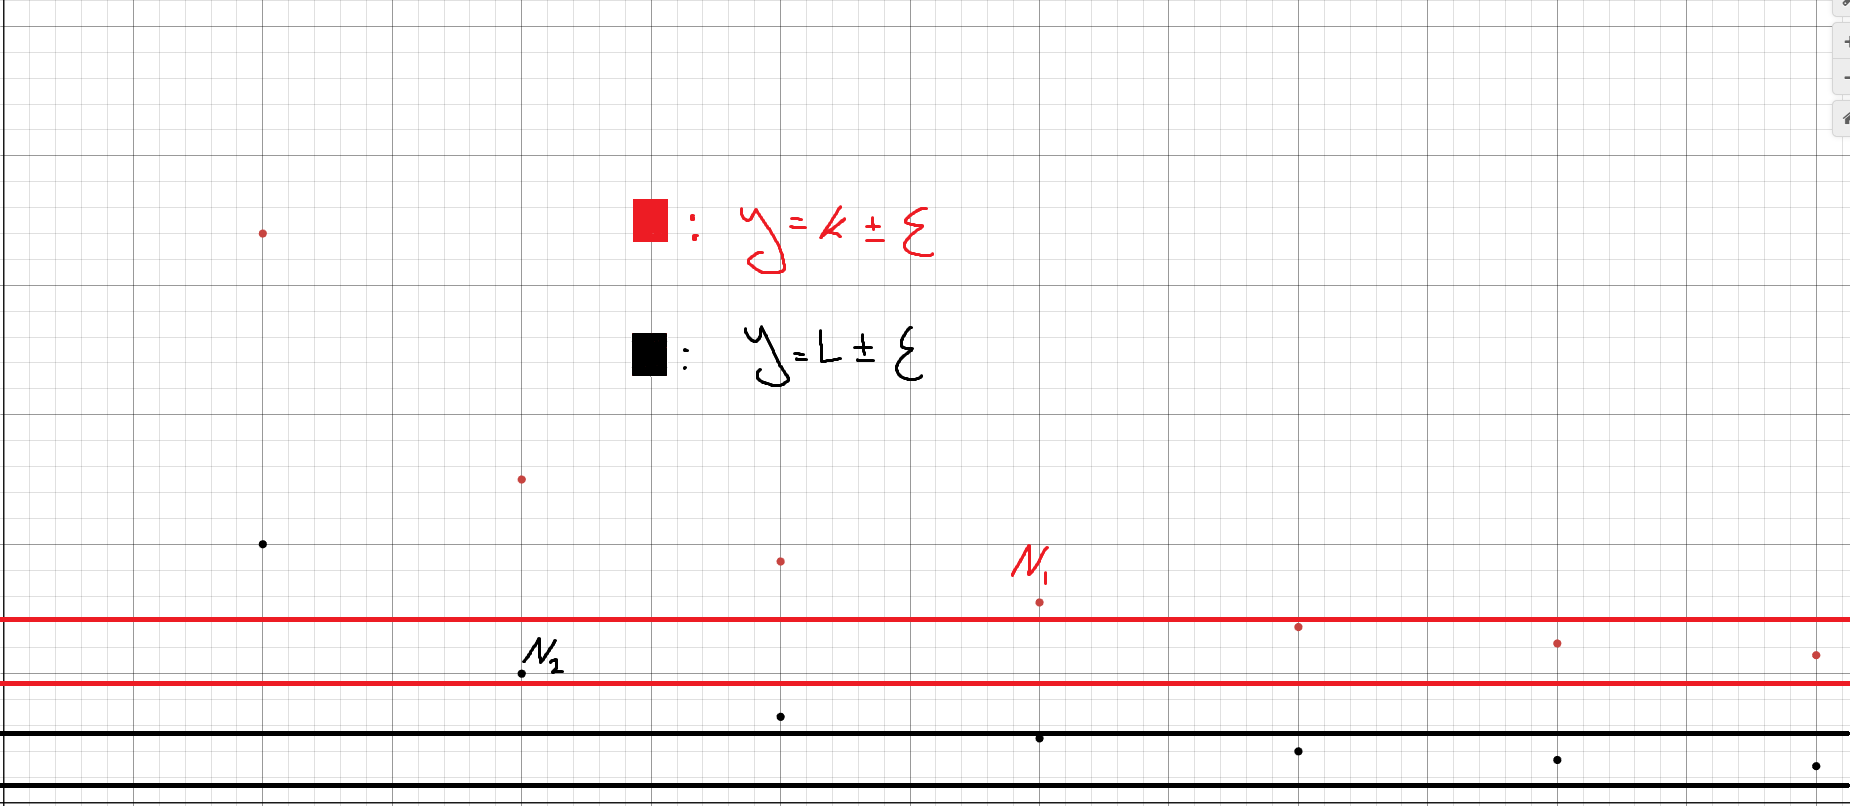
\includegraphics[scale=0.3]{pictures/UniqueLimitGraph.png}
\subsection{Mathematical Proof}
Given: $a_n\rightarrow K \Longrightarrow$\\
$\forall\; \varepsilon>0,\; \exists\; N_1,$ such that $\forall\;n>N_1\Longrightarrow$
\[
    |a_n-K|<\varepsilon\; \equiv K-\varepsilon<a_n<K+\varepsilon
\]
Given: $a_n\rightarrow L \Longrightarrow$\\
$\forall\; \varepsilon>0,\; \exists\; N_2,$ such that $\forall\;n>N_2\Longrightarrow$
\[
    |a_n-L|<\varepsilon\; \equiv L-\varepsilon<a_n<L+\varepsilon
\]
Becuase it works for every positive number $\varepsilon$ then it must work for $\frac{K-L}{3}$\\
$K>L\iff K-L>0\iff \frac{K-L}{3}>0$\\
For $\varepsilon =\frac{K-L}{3}\;\exists\; N=max\{N_1,N_2\}$ such that $\forall\; n>N\Longrightarrow$
\[
    K-\varepsilon<a_n<K+\varepsilon\; \equiv\; K-\frac{K-L}{3}<a_n<K+\frac{K-L}{3}
\]
\[
    \frac{3K}{3}-\frac{K-L}{3}<a_n<\frac{3K}{3}+\frac{K-L}{3}\; \equiv\; \frac{2K+L}{3}<a_n<\frac{4K-L}{3}
\]
\[
    \frac{2K+L}{3}<a_n<\frac{4K-L}{3}
\]
We know that this statment is true, because if we're looking for all indexes bigger than $max\{N_1,N_2\}$ then we're looking for all indexes bigger than $N_1$.\\
At the same time, we know that if we're looking at all the indexes bigger than $max\{N_1,N_2\}$, then we're looking for all the indexes bigger than $N_2\Longrightarrow$
\[
    L-\frac{K-L}{3}<a_n<L+\frac{K-L}{3}\; \equiv\; \frac{3L}{3}-\frac{K-L}{3}<a_n<\frac{3L}{3}+\frac{K-L}{3}
\]
\[
    \frac{4L-K}{3}<a_n<\frac{K+2L}{3}
\]
Given that $L<K \Longrightarrow \frac{K+2L}{3}<\frac{2K+L}{3}\Longrightarrow$
\[
    \frac{4L-K}{3}<a_n<\frac{K+2L}{3}<\frac{2K+L}{3}<a_n<\frac{4K-L}{3}
\]
Meaning for all the indexes bigger than $N$ the terms of the sequence are located in two different places, which is a contradiction.\\\\
\textbf{Note:} This is not an easy proof to grasp and understand, if you did not understand it at first, give it some time, go over it a couple of time, maybe sleep on it, but rest assured when you're reviewing the material in a couple of weeks, this proof is gonna be as smooth as butter.\\


\newpage

\section{Bounded Sequences}
\subsection{Definitions}
\begin{enumerate}
    \item A sequence $a_n$ is bounded from above $\iff \exists\; M\in \R,$ such that $\forall n\Longrightarrow a_n\leq M$
    \item A sequence $a_n$ is bounded from below $\iff \exists\; m\in \R,$ such that $\forall n\Longrightarrow m\leq a_n$
    \item A sequence $a_n$ is bounded $\iff$ it is bounded from above and below
\end{enumerate}

\subsubsection{Practice Question}
$a_n$ is bounded $\iff \exists\; K\in \R$ such that $\forall\; n \Longrightarrow |a_n|\leq K$\\
This is an identical question to the question in the \textbf{Groups} section that you should be able to solve on your own.\\

\subsection{Equivalent Definition For The Limit Of A Sequence}
$\forall\; \varepsilon>0,\; \exists\; N\in \N,$ such that $\forall n>N \Longrightarrow$
\[
    |a_n-L|<\varepsilon
\]
In the previous definition states that exists a real number $N$, but in this one it states that exists a natural number $N$, they're two different definition, we want to prove that they are equivalent.\\
\subsubsection{Floor/Ceiling Functions}
\[
    \lfloor x\rfloor = max\{m\in \Z\;|\; m\leq x\}
\]
\[
    \lceil x\rceil = min\{m\in \Z\;|\; m\geq x\}
\]
The Floor of $x,\; \lfloor x\rfloor$ returns the closest integer to $x$ from below\\
The Ceiling of $x,\; \lceil x\rceil$ returns the closest integer to $x$ from above\\
\textbf{Examples:}\\
\[
    \lfloor 5.4\rfloor = 5,\; \lfloor -3.2\rfloor = -4,\; \lfloor 3\rfloor = 3
\]
\[
    \lceil 5.4\rceil = 6,\; \lceil -3.2\rceil = -3,\; \lceil 3\rceil = 3
\]
\textbf{Features of $\lfloor x\rfloor,\; \lceil x\rceil$}\\
\[
    \lfloor x\rfloor\leq x \qquad x\leq\lceil x\rceil
\]
If we look at any real number $N\in \R,\; N\leq \lceil N\rceil,\; \lceil N\rceil\in \N$
Using the definition of a limit we know:\\
$\forall\: \varepsilon>0 \:, \exists \: N\in \R,$ such that $\forall \: n>N \Longrightarrow$\\
\[
    |a_n-L|<\varepsilon
\]
$\forall\; n>\lceil N\rceil$, meaning we're looking at the indexes bigger than $\lceil N\rceil\Longrightarrow N\leq\lceil N\rceil<n,\;$ meaning we're also looking at the indexes bigger than $N\Longrightarrow$\\
\[
    |a_n-L|<\varepsilon
\]

\noindent\textbf{Theorem:}\\
$a_n\rightarrow L \Longrightarrow a_n$ is bounded\\
\begin{proof}
    $a_n\rightarrow L \Longrightarrow \;\text{for } \varepsilon=1,\; \exists\; N\in \N,$ such that $\forall n>N\Longrightarrow$
    \[
        |a_n-L|<1 \iff L-1<a_n<L+1
    \]
    Since the sequence approaches $L$ this means that for any positive number $\varepsilon,\; \exists N\ldots$\\
    Therefor i can pick any positive number i want, and it is still going to work, because it works with any positive number.\\
    \textbf{Note:} You can pick any positive number instead of $1$ and the proof still works the same.\\
    If we look at the terms of the sequence:
    \[
        a_1,a_2,a_3,\ldots,a_N,a_{N+1},\ldots,a_n
    \]
    We know for a fact that forall indexes after $N$ the sequence is bounded because of the definition of the limit $\forall n>N\Longrightarrow L-1<a_n<L+1$\\
    That leaves us with the first $N$ terms, if we look at the group $\{a_1,a_2,\ldots,a_N\}$, it is finite group of real numbers, meaning it has a maximum and a minimum.\\
    \[
        K=max\{a_1,a_2,\ldots,a_N\},\; k = min\{a_1,a_2,\ldots,a_N\}
    \]
    $\forall\; 1\leq n\leq N \Longrightarrow k\leq a_n\leq K$, although the first $N$ terms are bounded, and all the terms after $N$th term are bounded as well, this does not prove that the sequence is bounded.\\
    \textbf{Reminder}:\\
    A sequence is bounded $\iff \exists\; m,M\: ,$ such that $\forall n\Longrightarrow m\leq a_n\leq M$\\
    Let $M = max\{K,L+1\}$ , $m = min\{k,L-1\}\Longrightarrow$\\
    \[
    \forall\; n \quad m\leq a_n\leq M
    \]
\end{proof}


\section{Limit Theorems}
\subsection{Limit Arithmetics}
Given: $a_n\rightarrow L,\; b_n\rightarrow K\Longrightarrow$
\begin{enumerate}
    \item $\forall c\in \R\Longrightarrow c\cdot a_n \rightarrow c\cdot L$
    \item $a_n+b_n\rightarrow L+K$
    \item $a_n\cdot b_n\rightarrow L\cdot K$
    \item If $k\neq0,\forall\; n\; b_n\neq 0 \Longrightarrow \frac{a_n}{b_n}\rightarrow \frac{L}{K}$
    \item $a_n\rightarrow L \Longrightarrow |a_n|\rightarrow |L|$
    \item $a_n\rightarrow 0 \iff |a_n|\rightarrow 0$
    \item $a_n\rightarrow L,\; L\geq 0,\; a_n\geq 0\; \forall\; n\Longrightarrow \sqrt{a_n}\rightarrow \sqrt{L}$
\end{enumerate}
\subsubsection{Proof 1}
We want to prove that $c\cdot a_n\rightarrow c\cdot L$ meaning:\\
We want to prove $\forall\; \varepsilon>0,\; \exists\; N\in \R,$ such that $\forall n>N\Longrightarrow$\\
\[
    |c\cdot a_n-c\cdot L|=|c\cdot(a_n-L)| = |c|\cdot|a_n-L|<\varepsilon
\]
\[
    \iff |a_n-L|<\frac{\varepsilon}{|c|} \quad \text{For\;} c\neq 0
\]
 
$a_n\rightarrow L\Longrightarrow \text{For}\; \frac{\varepsilon}{|c|},\; \exists\; N_1\in \R,$ such that $\forall n>N\Longrightarrow$
\[
    |a_n-L|<\frac{\varepsilon}{|c|}
\]
$\exists\; N=N_1$ such that $\forall n>N_1\Longrightarrow$
\[
    |c\cdot a_n-c\cdot L|<\varepsilon
\]
Remember the definition of a limit works for any positive number, we just named it $\varepsilon$ that's why we say $\forall\; \varepsilon>0$, as you can see $\frac{\varepsilon}{|c|}$ is a positive number, this is why we can pick it to be our positive number.\\
The theorem works for $c\neq 0$ although it states that $\forall\; c\in \R$, meaning we have to prove that it works for $c=0$.\\
For $c=0,\; 0\cdot a_n = 0$, the sequence $0\cdot a_n$ is a constant sequence and we proved $\forall\; c\in \R\; \lim_{n\to\infty} c = c \Longrightarrow 0\cdot a_n \rightarrow 0$\\

\subsubsection{Proof 2}
We want to prove $a_n+b_n\rightarrow L+K$\\
We want to prove that $\forall\; \varepsilon>0,\; \exists N\in \R,\;$ such that $\forall\; n>N\Longrightarrow$
\[
    |(a_n+b_n)-(L+K)|=|(a_n-L)+(b_n-K)|
\]
\[
    |(a_n-L)+(b_n-K)|\leq |a_n-L|+|b_n-K|<\varepsilon \quad \textbf{Feature 6}
\]
\[
    \iff |a_n-L|<\frac{\varepsilon}{2}\; \text{And\;} |b_n-K|<\frac{\varepsilon}{2}
\]
$a_n\rightarrow L\Longrightarrow$ For any positive number the definition of a limit works on it.\\
For $\frac{\varepsilon}{2}\; \exists\; N_1,\;$ such that $\forall n>N_1 \Longrightarrow$
\[
    |a_n-L|<\frac{\varepsilon}{2}
\]
$b_n\rightarrow K\Longrightarrow$ For any positive number the definition of a limit works on it.\\
For $\frac{\varepsilon}{2}\; \exists\; N_2,\;$ such that $\forall n>N_2 \Longrightarrow$
\[
    |b_n-K|<\frac{\varepsilon}{2}
\]
For $N=max\{N_1,N_2\},\;\forall\; n>N$ for all indexes bigger than $N$ are also bigger or equal to $N_1$ and $N_2\Longrightarrow$
\[
    |a_n-L|<\frac{\varepsilon}{2} \quad \text{And} \quad |b_n-K|<\frac{\varepsilon}{2}
\]


\subsubsection{Proof 3}
We want to prove that $a_n\cdot b_n\rightarrow L\cdot K$\\
We want to prove that $\forall\; \varepsilon>0,\; \exists\; N\in \R,\;$ such that $\forall\; n>N \Longrightarrow$
\[
    |a_n\cdot b_n -L\cdot K|= |a_n b_n-a_nK+a_nK-LK|
\]
\[
    |a_n b_n-a_nK+a_nK-LK| = |a_n(b_n-K)+K(a_n-L)|
\]
\[
    |a_n(b_n-K)+K(a_n-L)|\leq |a_n(b_n-K)|+|K(a_n-L)|\quad \textbf{Feature 6}
\]
\[
    |a_n(b_n-K)|+|K(a_n-L)|<\varepsilon
\]
We want to prove that $|a_n(b_n-K)|+|K(a_n-L)|<\varepsilon$ in order to do so we have to prove that $|a_n(b_n-K)|<\frac{\varepsilon}{2}$ and $|K(a_n-L)|<\frac{\varepsilon}{2}$\\
$a_n$ is convergent, that means that it is bounded, we proved earlier that every convergent sequence is bounded.\\
$\Longrightarrow \exists\; M\in \R\;$ such that $|a_n|<M$ and $|K|<M$ \textbf{You'll see why later}.\\
\[
    \Longrightarrow |a_n(b_n-K)|\leq |M(b_n-K)| = |M|\cdot|b_n-K|
\]
\[
   |M|\cdot|b_n-K|<\frac{\varepsilon}{2} \iff |b_n-K|<\frac{\varepsilon}{2M}
\]
This is what we want to prove, important to note that $\frac{\varepsilon}{2M}$ is positive.\\
$b_n\rightarrow K\;,$ Which is why we can say for $\frac{\varepsilon}{2M},\; \exists\; N_1\in \R,\;$ such that $\forall\; n>N_1\Longrightarrow$
\[
    |b_n-k|<\frac{\varepsilon}{2M}
\] 
\[
    |K(a_n-L)|= |K|\cdot |a_n-L|
\]
\[
    |K|\cdot |a_n-L|<\frac{\varepsilon}{2} \iff |M|\cdot|a_n-L|<\frac{\varepsilon}{2}
\]
\[
    |M|\cdot |a_n-L|<\varepsilon \iff |a_n-L|<\frac{\varepsilon}{2M}
\]
We could've continued to prove this theory without getting rid of the $K$, but if we haven't, we would've had to prove the case were $K = 0$\\
\textbf{What would've happened}:\\
\[
    |K|\cdot|a_n-L|<\frac{\varepsilon}{2} \iff |a_n-L|<\frac{\varepsilon}{2K}
\]
Which is true for $K\neq 0$, then we would have another proof for when $K=0$, now if we get a number $M$ which bigger than $|K|$, then this number $M$ is bigger than $0$, because $0\leq|K|<M \Longrightarrow 0<M$\\\\
We want to prove that $|a_n-L|<\frac{\varepsilon}{2M}$, important to note that $\frac{\varepsilon}{2M}$ is positive, $a_n\rightarrow L$, Which is why we can say\\
\noindent For $\frac{\varepsilon}{2M},\; \exists\; N_2\in \R,\;$ such that $\forall n>N_2\Longrightarrow$
\[
    |a_n-L|<\frac{\varepsilon}{2M}
\]
$\forall\; \varepsilon>0,\;\exists\; N=max\{N_1,N_2\},$ such that $\forall\; n>N\Longrightarrow$
\[
    |a_nb_n-LK|<\varepsilon
\]

\subsubsection{Proof 5}
We want to prove that $\forall\; \varepsilon>0,\;\exists\; N\in \R,\;$ such that $\forall\; n>N\Longrightarrow$
\[
    \Big| |a_n| - |L| \Big| \leq \Big| a_n-L \Big|<\varepsilon \quad \textbf{Feature 7}
\]
We want to prove that $|a_n-L|<\varepsilon$\\
$a_n\rightarrow L \Longrightarrow \forall\; \varepsilon>0,\; \exists N\in \R,\;$ such that $\forall n>N\Longrightarrow$
\[
    |a_n-L|<\varepsilon
\]

\subsubsection{Proof 7}
We want to prove $\sqrt{a_n}\rightarrow \sqrt{L}$, given that $L\geq 0,\; a_n\geq 0\; \forall\; n$\\
We want to prove that $\forall\; \varepsilon>0,\; \exists\; N\in \R,\;$ such that $\forall\; n>N\Longrightarrow$
\[
    |\sqrt{a_n}-\sqrt{L}|=\Big|\frac{(\sqrt{a_n}-\sqrt{L})\cdot (\sqrt{a_n}+\sqrt{L})}{\sqrt{a_n}+\sqrt{L}} \Big| = \Big|\frac{a_n-L}{\sqrt{a_n}+\sqrt{L}}\Big|
\] 
$a_n\geq 0 \; \forall\; n \Longrightarrow \sqrt{a_n}+\sqrt{L}\leq\sqrt{L}\iff \frac{1}{\sqrt{a_n}+\sqrt{L}}\leq\frac{1}{\sqrt{L}}\; \forall\; L\neq 0$
\[
    \Big|\frac{a_n-L}{\sqrt{a_n}+\sqrt{L}}\Big|\leq\Big|\frac{a_n-L}{\sqrt{L}}\Big| = \frac{|a_n-L|}{\sqrt{L}}
\]
\[
    \frac{|a_n-L|}{\sqrt{L}}<\varepsilon \iff |a_n-L|<\varepsilon\sqrt{L}
\]
For $\varepsilon\sqrt{L},\; \exists\; N\in \R,\;$ such that $\forall\; n>N\Longrightarrow$
\[
    |a_n-L|<\varepsilon\sqrt{L}
\]
We have to prove when $L=0$, we have to prove that $\forall\; \varepsilon>0,\; \exists\; N\in\R,\;$ such that $\forall\; n>N\Longrightarrow$
\[
    |\sqrt{a_n}-\sqrt{0}| = |\sqrt{a_n}| = \sqrt{a_n}
\]
\[
    \sqrt{a_n}<\varepsilon \iff a_n<\varepsilon^2
\]
For $\varepsilon^2,\; \exists\; N\in\R,\;$ such that $\forall n>N\Longrightarrow$
\[
    |a_n-0|=a_n<\varepsilon^2
\]

\newpage

\subsection{The 0 - Bounded Theorem}
Given: $a_n\rightarrow 0,\; b_n$ is bounded $\Longrightarrow a_nb_n\rightarrow 0$
\begin{proof}
    We want to prove $\forall\; \varepsilon>0,\; \exists\; N\in \R,\;$ such that $\forall\; n>N\Longrightarrow$
    \[
        |a_nb_n-0|=|a_nb_n| = |a_n|\cdot|b_n|<\varepsilon
    \]
    $b_n$ is bounded $\Longrightarrow$
    \[
        \exists\; M\in \R,\; \text{such that}\; |b_n|<M
    \]
    \[
        \Longrightarrow |a_n|\cdot |b_n|\leq M\cdot|a_n|
    \]
    \[
        M|a_n|<\varepsilon \iff |a_n|<\frac{\varepsilon}{M}
    \]
    Meaning we need to prove that $|a_n|<\frac{\varepsilon}{M}$, since $a_n\rightarrow 0$, for $\frac{\varepsilon}{M},\; \exists\; N\in \R,\;$ such that $\forall\; n>N\Longrightarrow$
    \[
        |a_n-0| = |a_n|<\frac{\varepsilon}{M}
    \] 
\end{proof}

\subsection{Sandwich Theorem}
Given: $\forall\; n\quad a_n\leq b_n\leq c_n,\;$ and $a_n\rightarrow L,\; c_n\rightarrow L \Longrightarrow b_n\rightarrow L$\\
$b_n\rightarrow L \iff \forall\; \varepsilon>0,\; \exists\; N\in \R,\;$ such that $\forall\; n>N \Longrightarrow$
\[
    |b_n-L|<\varepsilon
\]
This is what it means for a sequence to convergent to $L$, which is what we want to prove.\\
    $a_n\rightarrow L \Longrightarrow$\\
    $\forall\; \varepsilon>0,\;\exists\; N_1\in \R,\;$ such that $\forall\; n>N\Longrightarrow$
    \[
        |a_n-L|<\varepsilon \iff L-\varepsilon<a_n<L+\varepsilon
    \]
    $c_n\rightarrow L \Longrightarrow$\\
    $\forall\; \varepsilon>0,\;\exists\; N_2\in \R,\;$ such that $\forall\; n>N\Longrightarrow$
    \[
        |c_n-L|<\varepsilon \iff L-\varepsilon<c_n<L+\varepsilon
    \]
    $\forall\; n>N_1 \Longrightarrow$
    \[
        L-\varepsilon<a_n\leq b_n
    \]
    $\forall\; n>N_2 \Longrightarrow$
    \[
        b_n\leq c_n<L+\varepsilon
    \]
    $\exists\; N=max\{N_1,N_2\},\;$ such that $\forall\; n>N\Longrightarrow$
    \[
        L-\varepsilon<a_n\leq b_n\leq c_n<L+\varepsilon
    \]
    \[
        \Longrightarrow L-\varepsilon<b_n<L+\varepsilon
    \]

\newpage
\subsection{More Limit Thoerems}
\subsubsection{Theroem 1}
$a_n \rightarrow L>0 \Longrightarrow \exists\; N$, such that $\forall n>N \Longrightarrow a_n>0$\\
\[
    a_n \rightarrow L \Longrightarrow \forall\; \varepsilon >0,\; \exists\; N_1 \text{, such that } \forall\; n>N \Longrightarrow
    \]
\[        
    |a_n-L|<\varepsilon \iff L-\varepsilon<a_n<L+\varepsilon
\]
$L>0 \Longrightarrow \frac{L}{2}>0$, For $\varepsilon = \frac{L}{2},\; \exists\; N_1$, such that $\forall n>N_1 \Longrightarrow$
\[
    L-\frac{L}{2}<a_n<L+\frac{L}{2}
\]
\[
    0<\frac{L}{2}<a_n<\frac{3L}{2} \Longrightarrow a_n>0
\]
\subsubsection{Theorem 2}
$a_n\rightarrow L,\; b_n\rightarrow K ,\; \forall\; n\in \N\;\Longrightarrow a_n\geq b_n \Longrightarrow L\geq K$\\
Given two real numbers $L,K$ that we know nothing about, we know that one of two things is true:\\
\begin{enumerate}
    \item $L\geq K$
    \item $L<K$
\end{enumerate}
If we are able to prove that the statment $L<K$ is false, then we prove that $L\geq K$.\\
We're going to do a prove by contradiction, by assuming that something is true, then coming to a contradiction about what we know for a fact is true.\\\\
Let's assume that $L<K$\\
$a_n\rightarrow L \Longrightarrow \forall\; \varepsilon >0, \exists\; N,$ such that $\forall\; n>N \Longrightarrow$\\
\[
    L-\varepsilon<a_n<L+\varepsilon
\]
$b_n\rightarrow L \Longrightarrow \forall\; \varepsilon >0, \exists\; N,$ such that $\forall\; n>N \Longrightarrow$\\
\[
    L-\varepsilon<b_n<L+\varepsilon
\]
Given: $K-L>0 \iff \frac{K-L}{3}>0 \Longrightarrow$ For $\varepsilon = \frac{K-L}{3}\; \exists\; N_1$ such that $\forall\; n>N_1\Longrightarrow$\\
\[
    L-\frac{K-L}{3}<a_n<\L+\frac{K-L}{3}
\] 
\[
    a_n<\frac{K+2L}{3}
\]
$\exists\; N_2$ such that $\forall\; n>N_2 \Longrightarrow$\\
\[
    K-\frac{K-L}{3}<b_n<K+\frac{K-L}{3}
\]
\[
    \frac{2K+L}{3}<b_n
\]
$K>L \Longrightarrow \frac{K+2L}{3}<\frac{2K+L}{3}\Longrightarrow$ For $N = max\{N_1,N_2\}$ and $\forall\; n>N\Longrightarrow$\\
\[
    a_n<\frac{K+2L}{3}<\frac{2K+L}{3}<b_n
\]
Which is a contradiction to the statment that $a_n\geq b_n \forall\; n\in \N$, meaning that the statment $L<K$ is not true. that means that the statment $L\geq K$ is true.\\
\subsection{Harmonic, Geometric, Arithmetic Mean}
\subsubsection{Definitions}
\textbf{Arithmetic Mean}\\
Given a set of real numbers $\{x_1,x_2,x_3,\ldots,x_n\}$, the arithmetic mean of this set is:\\
\[
    \frac{x_1+x_2+x_3+\ldots+x_n}{n}
\]
\textbf{Geometric Mean}\\
Given a set of positive numbers $\{y_1,y_2,y_3,\ldots,y_n\}$, the geometric mean of this set is:\\
\[
    \sqrt[n]{y_1\cdot y_2\cdot y_3\cdot \;\ldots\; \cdot  y_n}
\]
\textbf{Harmonic Mean}\\
Given a set of positive numbers $\{z_1,z_2,z_3,\ldots,z_n\}$, the harmonic mean of this set is:\\
\[
    \frac{n}{\frac{1}{z_1}+\frac{1}{z_2}+\frac{1}{z_3}+\ldots+\frac{1}{z_n}}
\]
\subsubsection{Inequalities}
\[
    \text{Harmonic Mean } \leq \text{Geometric Mean } \leq \text{Arithmetic Mean}
\]
In Short:\\
\[
    \text{HM GM AM Inequalities}
\]
Given a set of positive numbers $\{x_1,x_2,x_3,\ldots,x_n\}$\\
\[
    \frac{n}{\frac{1}{x_1}+\frac{1}{x_2}+\frac{1}{x_3}+\ldots+\frac{1}{x_n}} \leq \sqrt[n]{x_1\cdot x_2\cdot x_3\cdot\; \ldots\; \cdot x_n} \leq \frac{x_1+x_2+x_3+\ldots+x_n}{n}
\]
\subsubsection{GM AM Inequality Proof}
We will prove this inequality using induction.\\
Base Case:\\
For $n = 1\;$ $\frac{x_1}{1} = {x_1}^1$ we're more interested when $n = 2$\\
For $n = 2\;$
\[
    \sqrt[2]{x_1\cdot x_2} \leq \frac{x_1+x_2}{2}
\]
\[
    \Updownarrow 
\]
\[
    x_1\cdot x_2 \leq \frac{(x_1+x_2)^2}{4} = \frac{{x_1}^2+2x_1x_2+{x_2}^2}{4}
\]
\[
    \Updownarrow
\]
\[
    4x_1x_2\leq {x_1}^2+2x_1x_2+{x_2}^2
\]
\[
    \Updownarrow
\]
\[
    0\leq {x_1}^2-2x_1x_2+{x_2}^2
\]
$(x_1-x_2)^2 = {x_1}^2-2x_1x_2+{x_2}^2$
\[
    \Updownarrow
\]
\[
    0\leq (x_1-x_2)^2
\]
Which is always true.\\
Let's assume that for any natural number $k\geq 2$ that the claim, we want to prove that the claim is also true for $2k$, Meaning:\\
\[
    \sqrt[2k]{x_1\cdot x_2\cdot x_3\cdot\; \ldots\; x_{2k}}\leq \frac{x_1+x_2+x_3+\ldots+x_{2k}}{2k}
\]
Using our induction assumption that:\\
\[
    \sqrt[k]{x_1\cdot x_2\cdot x_3\cdot\; \ldots\; x_{k}}\leq \frac{x_1+x_2+x_3+\ldots+x_{k}}{k}
\]
We can see that:\\
\[
    \frac{x_1+x_2+x_3+\ldots+x_{2k}}{2k} = \frac{\frac{x_1+x_2+x_3+\ldots+x_{k}}{k}+\frac{x_{k+1}+x_{k+2}+x_{k+3}+\ldots+x_{2k}}{k}}{2}
\]
\[
    \frac{\frac{x_1+x_2+x_3+\ldots+x_{k}}{k}+\frac{x_{k+1}+x_{k+2}+x_{k+3}+\ldots+x_{2k}}{k}}{2}\geq \frac{\sqrt[k]{x_1\cdot x_2\cdot x_3\; \cdot\;x_k} + \sqrt[k]{x_{k+1}\cdot x_{k+2}\cdot x_{k+3}\cdot \ldots x_{2k}}}{2}
\]
\[
    \frac{\sqrt[k]{x_1\cdot x_2\cdot x_3\; \cdot\;x_k} + \sqrt[k]{x_{k+1}\cdot x_{k+2}\cdot x_{k+3}\cdot \ldots x_{2k}}}{2} \geq \sqrt{\sqrt[k]{x_1\cdot x_2\cdot x_3\; \cdot\;x_k}\cdot \sqrt[k]{x_{k+1}\cdot x_{k+2}\cdot x_{k+3}\cdot \ldots x_{2k}}}
\]
\[
    \sqrt{\sqrt[k]{x_1\cdot x_2\cdot x_3\; \cdot\;x_k}\cdot \sqrt[k]{x_{k+1}\cdot x_{k+2}\cdot x_{k+3}\cdot \ldots x_{2k}}} = \sqrt{\sqrt[k]{x_1\cdot x_2\cdot x_3\cdot \ldots\cdot x_k\cdot \ldots x_{2k}}}
\]
\[
    \sqrt{\sqrt[k]{x_1\cdot x_2\cdot x_3\cdot \ldots\cdot x_k\cdot \ldots x_{2k}}} = \sqrt[2k]{x_1\cdot x_2\cdot x_3\cdot \ldots\cdot x_k\cdot \ldots x_{2k}}
\]
We proved that if we know that $P(k)$ is true, then $P(2k)$ is true.\\
Meaning: $P(2)$ is true (We Proved It In Base Case), then $P(4)$ is also true, then $P(8)$ is true, then $P(16)$ is also true $\ldots$, it is not quite a full proof because what about $P(3)$ and $P(5),\;P(6) \ldots$ , our second step will fill in the gaps.\\
We're still on our induction assumption that $P(k)$ is true.\\
we want to prove that $P(k-1)$ is true.\\
From our induction assumption we know that:
\[
    \frac{x_1+x_2+x_3+\ldots+x_k}{k}\geq \sqrt{x_1\cdot x_2\cdot x_3\cdot \; \ldots\; \cdot x_k}
\]
Note that this inequality is true when $x_n$ is any positive number, meaning i can pick any specified number instead of $x_n$, and this inequality will still be true.\\
Let $x_k = \frac{x_1+x_2+x_3+\ldots x_{k-1}}{k-1}$
\[
    \frac{x_1+x_2+x_3+\ldots+x_k}{k} = \frac{x_1+x_2+x_3+\ldots+\frac{x_1+x_2+x_3+\ldots x_{k-1}}{k-1}}{k}
\]
\[
    \frac{x_1+x_2+x_3+\ldots+x_{k-1}+\frac{x_1+x_2+x_3+\ldots x_{k-1}}{k-1}}{k} \geq \sqrt[k]{x_1\cdot x_2\cdot x_3\cdot \;\ldots\; \cdot \frac{x_1+x_2+x_3+\ldots x_{k-1}}{k-1}}
\]
\[
    \frac{x_1+x_2+x_3+\ldots+x_{k-1}}{k-1} \leq x_1+x_2+x_3+\ldots+x_{k-1} 
\]
\[
    \Longrightarrow \frac{x_1+x_2+x_3+\ldots+x_{k-1}+\frac{x_1+x_2+x_3+\ldots x_{k-1}}{k-1}}{k} \leq \frac{x_1+x_2+x_3+\ldots+x_{k-1}}{k-1}
\]
\[
    \frac{x_1+x_2+x_3+\ldots+x_{k-1}}{k-1} \geq \sqrt[k]{x_1\cdot x_2\cdot x_3\cdot \;\ldots\; \cdot \frac{x_1+x_2+x_3+\ldots x_{k-1}}{k-1}}
\]
Power both sides by k
\[
    {(\frac{x_1+x_2+x_3+\ldots+x_{k-1}}{k-1})}^k \geq x_1\cdot x_2\cdot x_3\cdot \;\ldots\; \cdot \frac{x_1+x_2+x_3+\ldots x_{k-1}}{k-1}
\]
Dividing both sides by $\frac{x_1+x_2+x_3+\ldots+x_{k-1}}{k-1}$
\[
    \frac{{(\frac{x_1+x_2+x_3+\ldots+x_{k-1}}{k-1})}^k}{\frac{x_1+x_2+x_3+\ldots+x_{k-1}}{k-1}} \geq \frac{x_1\cdot x_2\cdot x_3\cdot \;\ldots\; \cdot \frac{x_1+x_2+x_3+\ldots x_{k-1}}{k-1}}{\frac{x_1+x_2+x_3+\ldots x_{k-1}}{k-1}}
\]
\[
    {(\frac{x_1+x_2+x_3+\ldots+x_{k-1}}{k-1})}^{k-1} \geq x_1\cdot x_2\cdot x_3\cdot \;\ldots\; \cdot x_{k-1}
\]
k'th root both sides
\[
    \frac{x_1+x_2+x_3+\ldots+x_{k-1}}{k-1} \geq \sqrt[k-1]{x_1\cdot x_2\cdot x_3\cdot \;\ldots\; \cdot x_{k-1}}
\]
Which is what we wanted to prove.\\
If we know that $P(k)$ is true, then $P(k-1)$ is true.\\
Meaning that $P(2)$ is true, then $P(4)$ is true based on our previous proof,$P(4)$ is true, then $P(3)$ is true, then $P(6)$ is true, then $P(5)$ is true, then $P(10)$ is true, then $P(9)$ is true, and if $P(4)$ is true, then $P(8)$ is true and $P(7)$ is true.\\
Meaning for all natural numbers the inequality above is true.\\
\subsubsection{HM GM Inequality Proof}
Just to remember that the Harmonic Mean is:
\[
    \frac{n}{\frac{1}{x_1}+\frac{1}{x_2}+\frac{1}{x_3}+\ldots+\frac{1}{x_n}}
\]
We want to prove that:
\[
    \frac{n}{\frac{1}{x_1}+\frac{1}{x_2}+\frac{1}{x_3}+\ldots+\frac{1}{x_n}}\leq \sqrt[n]{x_1\cdot x_2\cdot x_3\cdot\;\ldots\; \cdot x_n}
\]
For any positive number $x_n, \frac{1}{x_n},\; \forall\; n\in \N$ is also positive, let's define $a_n$ to be the fraction $\frac{1}{x_n}$.\\
We know:
\[
    \sqrt[n]{a_1\cdot a_2\cdot a_3\cdot\;\ldots\;\cdot a_n}\leq \frac{a_1+a_2+a_3+\ldots+a_n}{n}
\]
Let's take the inverse of both sides
\[
    \frac{1}{\sqrt[n]{a_1\cdot a_2\cdot a_3\cdot\;\ldots\;\cdot a_n}} \geq \frac{n}{a_1+a_2+a_3+\ldots+a_n}
\]
Substitute $\frac{1}{x_n}$ for $a_n$
\[
    \frac{1}{\sqrt[n]{\frac{1}{x_1}\cdot \frac{1}{x_2}\cdot \frac{1}{x_3}\cdot\;\ldots\;\cdot \frac{1}{x_n}}} \geq \frac{n}{\frac{1}{x_1}+\frac{1}{x_2}+\frac{1}{x_3}+\ldots+\frac{1}{x_n}}
\]
\[
    \frac{1}{\sqrt[n]{\frac{1}{x_1}\cdot \frac{1}{x_2}\cdot \frac{1}{x_3}\cdot\;\ldots\;\cdot \frac{1}{x_n}}} = \frac{1}{\sqrt[-n]{x_1\cdot x_2\cdot x_3\cdot\; \ldots\; \cdot x_n}} = \sqrt[n]{x_1\cdot x_2\cdot x_3\cdot\; \ldots\; \cdot x_n}
\]
\[
    \sqrt[n]{x_1\cdot x_2\cdot x_3\cdot\; \ldots\; \cdot x_n} \geq   \frac{n}{\frac{1}{x_1}+\frac{1}{x_2}+\frac{1}{x_3}+\ldots+\frac{1}{x_n}}
\]
With that we proved that the Harmonic Mean $\leq$ the Geometric Mean.\\
Meaning:
\[
    \frac{n}{\frac{1}{x_1}+\frac{1}{x_2}+\frac{1}{x_3}+\ldots+\frac{1}{x_n}}\leq \sqrt[n]{x_1\cdot x_2\cdot x_3\cdot\; \ldots\; \cdot x_n}\leq \frac{x_1+x_2+x_3+\ldots x_n}{n}
\]
\subsection{Even More Limit Theorems}
Given $a_n \rightarrow L,\; a_n>0 \;\forall\; n\in \N \;$ We want to prove the following statments:\\
\begin{enumerate}
    \item The sequence of Arithmetic Mean $x_n = \frac{a_1+a_2+a_3+\ldots+a_n}{n} \rightarrow L$
    \item The sequence of Geometric Mean $y_n = \sqrt[n]{a_1\cdot a_2\cdot a_3\cdot\; \ldots\;\cdot a_n} \rightarrow L$
    \item The sequence of Harmonic Mean $z_n = \frac{n}{\frac{1}{a_1}+\frac{1}{a_2}+\frac{1}{a_3}+\ldots+\frac{1}{a_n}}\rightarrow L$
\end{enumerate}
\subsubsection{Proof 1}
$a_n\rightarrow L \iff \forall\; \varepsilon>0,\; \exists N_1\in \N$ such that $\forall\; n>N\Longrightarrow$
\[
    |a_n-L|<\frac{\varepsilon}{2}
\]
\[
    \big|\frac{a_1+a_2+a_3+\ldots+a_n}{n}-L \big| = \big|\frac{a_1+a_2+a_3+\ldots+a_n -nL}{n} \big| 
\]
\[
    \big|\frac{a_1+a_2+a_3+\ldots+a_n -nL}{n} \big| = \big|\frac{(a_1-L)+(a_2-L)+(a_3-L)+\ldots+(a_{N_1}-L)+\ldots+(a_n-L)}{n} \big|
\]
\[
    =
\]
\[
 \big|\frac{(a_1-L)+(a_2-L)+(a_3-L)+\ldots+(a_{N_1}-L)}{n}+\frac{(a_{N_1+1}-L)+(a_{N_1+2}-L)+(a_{N_1+3}-L)+\ldots+(a_n-L)}{n} \big|
\]
\[
    \leq
\]
\[
    \big|\frac{(a_1-L)+(a_2-L)+(a_3-L)+\ldots+(a_{N_1}-L)}{n}\big| + \big| \frac{(a_{N_1+1}-L)+(a_{N_1+2}-L)+(a_{N_1+3}-L)+\ldots+(a_n-L)}{n} \big|
\]
Let $a_1+a_2+a_3+\ldots+a_{N_1} - N_1\cdot L = t\;$ which is a constant, because we know what the values of $a_1,\ldots a_{N_1}$ are, and $N_1$ and $L$\\

If we look at the sequence $\frac{t}{n}$ we can see that it approaches $0$, therefor\\
$\forall\; \varepsilon>0,\; \exists N_2$ such that $\forall\; n>N_2 \Longrightarrow$
\[
    \big|\frac{(a_1-L)+(a_2-L)+(a_3-L)+(a_{N_1}-L)}{n}\big| = \big|\frac{t}{n} \big| <\frac{\varepsilon}{2} 
\]
We know that $\forall\; n>N_1 \Longrightarrow |a_n-L|<\varepsilon$ 
\[
    \big|\frac{(a_{N_1+1}-L)+(a_{N_1+2}-L)+(a_{N_1+3}-L)+\ldots+(a_n-L)}{n} \big|\leq \big|a_{N_1+1}-L\big| + \big|a_{N_1+2}-L\big| + \ldots + \big|a_n-L\big| \cdot \frac{n-N_1}{n}
\]
\[
    \frac{n-N_1}{n}<\frac{n}{n} = 1
\]
\[
    \big|a_{N_1+1}-L\big| + \big|a_{N_1+2}-L\big| + \ldots + \big|a_n-L\big| \cdot \frac{n-N_1}{n} < \frac{\varepsilon}{2}\cdot \frac{n-N_1}{n} <\frac{\varepsilon}{2}
\]
For $N = max\{N_1,N_2\}$
\[
    |x_n-L|<\varepsilon
\]
\subsubsection{Proof 3}
Let $c_n = \frac{1}{a_n} \Longrightarrow c_n\rightarrow L$
\[
    \text{Let } t_n = \frac{c_1+c_2+c_3+\ldots+c_n}{n} \rightarrow \frac{1}{L}
\]
Let $z_n = \frac{1}{t_n}\Longrightarrow z_n\rightarrow L$
\[
    z_n = \frac{n}{c_1+c_2+c_3+\ldots+c_n} = \frac{n}{\frac{1}{a_1}+\frac{1}{a_2}+\frac{1}{a_3}+\ldots+\frac{1}{a_n}}\rightarrow L
\]
\subsubsection{Proof 2}
We know about the HM GM AM Inequalities
\[
    \frac{n}{\frac{1}{a_1}+\frac{1}{a_2}+\frac{1}{a_3}+\ldots+\frac{1}{a_n}}\leq \sqrt[n]{a_1\cdot a_2\cdot a_3\cdot\; \ldots \; a_n} \leq \frac{a_1+a_2+a_3+\ldots+a_n}{n}
\]
We just proved these two limits
\[
    \frac{n}{\frac{1}{a_1}+\frac{1}{a_2}+\frac{1}{a_3}+\ldots+\frac{1}{a_n}} \rightarrow L
\]
\[
    \frac{a_1+a_2+a_3+\ldots+a_n}{n}\rightarrow L
\]
Using Sandwich Theorem
\[
    L\leq\sqrt[n]{a_1\cdot a_2\cdot a_3\cdot\; \ldots \; a_n}\leq L
\]
$\Longrightarrow \sqrt[n]{a_1\cdot a_2\cdot a_3\cdot\; \ldots \; a_n}\rightarrow L$
\subsubsection{Ratio Test Theorem}
If $a_n>0\; \forall\; n\in \N,\; \lim_{n\to\infty} \frac{a_{n}}{a_{n-1}} = L \Longrightarrow \sqrt[n]{a_n} = L$\\
Important to note that we don't know that $a_n\rightarrow L$\\
Let's define $a_0$ to be $1$\
\[
    a_n = \frac{a_1}{a_0}\cdot \frac{a_2}{a_1}\cdot\frac{a_3}{a_2}\cdot\frac{a_4}{a_3}\cdot\;\ldots\;\cdot \frac{a_n}{a_{n-1}}
\]
\[
    \sqrt[n]{a_n} = \sqrt[n]{\frac{a_1}{a_0}\cdot \frac{a_2}{a_1}\cdot\frac{a_3}{a_2}\cdot\frac{a_4}{a_3}\cdot\;\ldots\;\cdot \frac{a_n}{a_{n-1}}}
\]
Let $b_n = \frac{a_n}{a_{n-1}}$, we know that $b_n\rightarrow L$\\
\[
    \sqrt[n]{a_n} = \sqrt[n]{\frac{a_1}{a_0}\cdot \frac{a_2}{a_1}\cdot\frac{a_3}{a_2}\cdot\frac{a_4}{a_3}\cdot\;\ldots\;\cdot \frac{a_n}{a_{n-1}}} = \sqrt[n]{b_1\cdot b_2\cdot b_3\cdot \; \ldots \;b_n}
\]
We just proved that if $b_n>0\; \forall\; n\in N$ and $b_n\rightarrow L \Longrightarrow \sqrt[n]{b_1\cdot b_2\cdot b_3\cdot \; \ldots \;b_n}\rightarrow L$
\[
    \sqrt[n]{a_n} = \sqrt[n]{b_1\cdot b_2\cdot b_3\cdot \; \ldots \;b_n}\rightarrow L
\]
\subsubsection{Theorem Applications}
We want to prove that given $c>0$ $\sqrt[n]{c} \rightarrow 1$\\
$a_n = c \Longrightarrow \lim_{n\to\infty} \frac{a_n}{a_{n-1}} = \frac{c}{c} = 1 \Longrightarrow \sqrt[n]{a_n} = 1 = \sqrt[n]{c}$\\
With the same concept we find the limit for the sequence $\sqrt[n]{n},\;$ let $a_n = n$\\
$\lim_{n\to\infty} \frac{a_n}{a_{n-1}} = \frac{n}{n-1}\rightarrow 1 \Longrightarrow \sqrt[n]{n} = 1$


\newpage
\section{Approaching $\infty$ and $-\infty$}
\subsection{Understanding The Definition}
We say that a sequence approaches $\infty$ if and only if we pick any real number, there exists a point  such that for all the indexes bigger than that point all the terms of the sequence are bigger than that number.\\
\subsection{The Definition}
$a_n\rightarrow \infty \iff \forall\; M\in \R,\; \exists\;N\in \R$, such that $\forall n>N \Longrightarrow$\\
\[
    a_n>M
\]
Proving that the sequence $a_n=n \rightarrow \infty$\\
$\forall\; M\in \R,\; \exists\; N=\square$, such that $\forall n>N\Longrightarrow$
\[
    n>N=M
\]
\subsection{Equivalent Definition}
$a_n\rightarrow \infty \iff \forall\;M>0,\;\exists\; N\in \R$, such that $\forall\; n>N\Longrightarrow$
\[
    a_n>M
\]
We can't just say that this is an equivalent definition for a sequence approaching infinity, we have to prove it.\\
Meaning we have to prove:\\
$\forall\; M\in \R,\; \exists\;N\in \R$, such that $\forall n>N \Longrightarrow a_n>M \iff a_n\rightarrow \infty \iff \forall\;M>0,\;\exists\; N\in \R$, such that $\forall\; n>N\Longrightarrow a_n>M$\\
$\Longrightarrow$\\
If we know that the definition works $\forall\; M\in \R$, then it works $\forall\;M>0$\\
$\Longleftarrow$\\
If we know that $\forall\; M>0,\;\exists\; \N\in\R$, such that $\forall\; n>N \Longrightarrow$
\[
    a_n>M>0
\]
then it works $\forall\; M\leq 0$\\
You'll see why this is important.\\
\subsection{Definitions For Approaching $-\infty$}
Similarly $a_n\rightarrow -\infty \iff \forall\; M\in \R,\;$ or $\forall\; M>0,\; \exists\; N\in \R$, such that $\forall\; n>N\Longrightarrow$
\[
    a_n<M
\] 
\subsection{Proving $2^n\rightarrow \infty$}
$\forall\; M\in \R,\; \exists\; N=\square$, such that $\forall\; n>N\Longrightarrow$
\[
    2^n>2^N = M
\]
meaning that $N = \log_2 {M}$, the problem with this statment is that $M$ could be any number including negative numbers, which is a problem because $\log_2{x}$ is defined when $x>0$, this is we another definition for approaching infinity,  $\forall\;M>0.$\\
This is also true $\forall\; a>1$ meaning $a^n \rightarrow \infty$ \textbf{Prove As Practice}
\subsection{Infinity Limit Theorems}
$a_n\rightarrow \infty, a_n\neq 0 \;\forall\; n \Longrightarrow \frac{1}{a_n}\rightarrow 0$
We want to prove that $\forall\; \varepsilon>0\; \exists\; N$, such that $\forall\; n>N\Longrightarrow$
\[
    |\frac{1}{a_n} - 0| = |\frac{1}{a_n}|<\varepsilon
\]
\[
    \Updownarrow
\]
\[
    |a_n|>\frac{1}{\varepsilon}
\]
$a_n\rightarrow \infty \Longrightarrow$ For $M=\frac{1}{\varepsilon},\; \exists\;N_1$, such that $\forall\; n>N_1$
\[
    a_n>\frac{1}{\varepsilon}
\]
For $N=N_1$, such that $\forall\; n>N_1\Longrightarrow$
\[
    a_n>\frac{1}{\varepsilon} \Longrightarrow |a_n|>\frac{1}{\varepsilon}
\]
Given: $a_n\rightarrow 0, a_n>0\; \forall\; n\Longrightarrow \frac{1}{a_n}\rightarrow \infty$\\
We want to prove that $\forall\; M>0,\; \exists\;N$, such that $\forall\; n>N\Longrightarrow$
\[
    \frac{1}{a_n}>M \iff a_n<\frac{1}{M}
\]
$a_n\rightarrow 0 \Longrightarrow$ For $\varepsilon = \frac{1}{M}\Longrightarrow \exists\; N_1$, such that $\forall\; n>N_1\Longrightarrow$
\[
    |a_n-0| = |a_n| = a_n<\frac{1}{M}
\]
Given $|q|<1 \Longrightarrow |q|^n\rightarrow 0$\\
If $q = 0$, then $0^n \rightarrow 0$\\
Otherwise, for $q\neq 0 \Longrightarrow$ if $|q|<1 \Longrightarrow \frac{1}{|q|}>1$.\\
Let's define $a = \frac{1}{|q|}\Longrightarrow a>1 \Longrightarrow a^n \rightarrow \infty \Longrightarrow \frac{1}{a_n} = |q|^n \rightarrow 0$\\
\subsubsection{The Pizza Theroem}
Given: $a_n\leq b_n\; \forall\;n,\; a_n\rightarrow\infty\Longrightarrow b_n\rightarrow \infty$
$a_n\rightarrow \infty \Longrightarrow \forall\; M\in \R,\; \exists\; N_1$, such that $\forall\; n>N_1 \Longrightarrow$
\[
    a_n>M
\]
Given: $a_n\leq b_n \rightarrow$
\[
    M<a_n\leq b_n \Longrightarrow M<b_n
\]
Meaning that $b_n\rightarrow\infty$